\chapter{SYSTEM ARCHITECTURE}

\begingroup
\hyphenpenalty=10000
\exhyphenpenalty=10000
\sloppy

\section{OVERVIEW OF THE PROPOSED SYSTEM}

The proposed system presents a queuing-theory-based intelligent autoscaling framework designed to efficiently manage dynamic workloads in a microservices-based environment. Unlike traditional autoscaling approaches that rely on static CPU and memory thresholds, the proposed system utilizes real-time performance metrics and analytical modeling to make accurate and proactive scaling decisions.

The architecture is composed of five primary layers: request handling layer, microservices layer, monitoring and metrics collection layer, autoscaling decision engine, and traffic routing layer. Incoming user requests are first processed through an NGINX gateway, which routes traffic to appropriate backend services. Each microservice processes requests independently and generates performance metrics.

These metrics are collected using Prometheus and include request arrival rate, response latency, and throughput. The autoscaling engine processes these metrics to compute key queuing parameters such as arrival rate ($\lambda$), service rate ($\mu$), utilization ($\rho$), and mean response time ($W$). Based on these parameters, the Multistage Fine-Grained Dynamic Scaling (MFDS) mechanism determines scaling actions, while Microservice Scaling Optimization (MSO) calculates the optimal number of replicas. Fair Probabilistic Routing (FPR) ensures efficient load distribution across services, resulting in improved performance and resource utilization.

\begin{figure}[h]
    \centering
    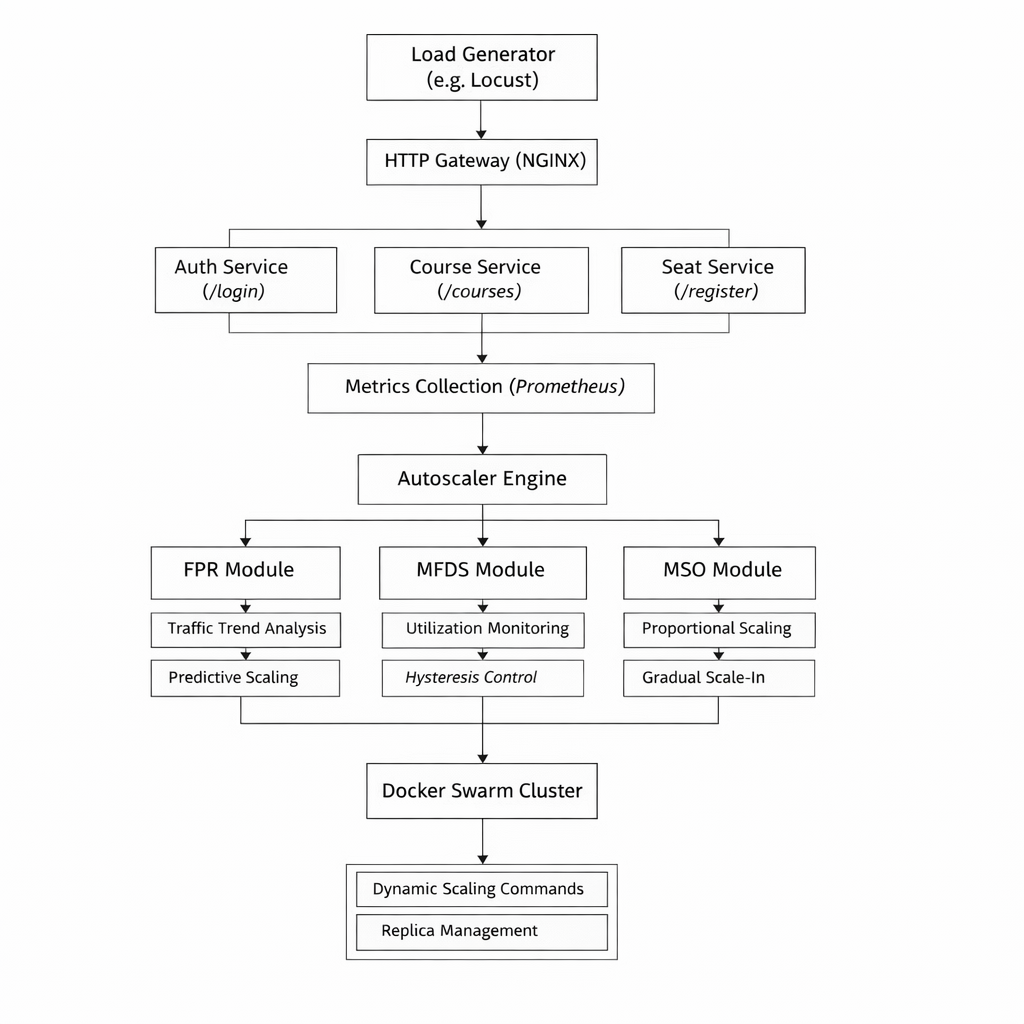
\includegraphics[width=0.9\linewidth]{3/Overall.png}
    \caption{Overall Architecture}
    \label{fig:sample}
\end{figure}

\section{DATA ACQUISITION LAYER}

The data acquisition layer plays a crucial role in collecting real-time system metrics required for intelligent autoscaling decisions. Unlike traditional systems that depend on static datasets, the proposed framework operates entirely on live traffic generated by actual user requests, ensuring that scaling decisions are based on current system state rather than outdated information.

Prometheus is employed as the primary monitoring tool to continuously collect comprehensive metrics from each microservice in the distributed architecture. These metrics include request arrival rate (requests per second), average service latency, total request count over time windows, and individual service response times across different endpoints. The collected data is stored in Prometheus's time-series database and processed at regular intervals (typically every 15-30 seconds) to ensure up-to-date system analysis while maintaining computational efficiency.

The raw metrics undergo transformation into queuing-theory-based parameters that form the foundation of the intelligent autoscaling algorithm. These include arrival rate ($\lambda$) representing the frequency of incoming requests, service rate ($\mu$) indicating the processing capacity of each service instance, utilization factor ($\rho = \lambda/\mu$) showing the current load intensity, and expected response time ($W$) calculated using queuing formulas. These parameters provide a more accurate representation of system behavior compared to traditional resource-based metrics like CPU and memory utilization.

This comprehensive data acquisition layer ensures that the autoscaling system operates on real-time, reliable, and mathematically meaningful data for decision-making, enabling precise performance predictions and optimal scaling actions.


\section{AUTOSCALING DECISION ENGINE}
 
The autoscaling decision engine is the core component responsible for determining scaling actions based on real-time system analysis. It utilizes the Multistage Fine-Grained Dynamic Scaling (MFDS) mechanism, which evaluates system performance based on multiple queuing theory parameters rather than simple resource utilization metrics.

Each microservice is modeled as an M/M/c queue, representing a multi-server queuing system where requests arrive according to a Poisson process and are served with exponentially distributed service times. The system computes key performance indicators including expected response time ($W$), system utilization ($\rho$), and average queue length ($L_q$) using established queuing theory formulas. These calculated values are compared against predefined SLA thresholds to determine whether scaling actions are required.

The decision logic operates on a multi-threshold approach: if the predicted response time exceeds the upper SLA threshold, the system triggers scale-out operations to add additional service replicas; if the response time falls below the lower threshold and utilization is sufficiently low, scale-in operations are initiated to reduce resource allocation.

\begin{figure}[h]
\centering
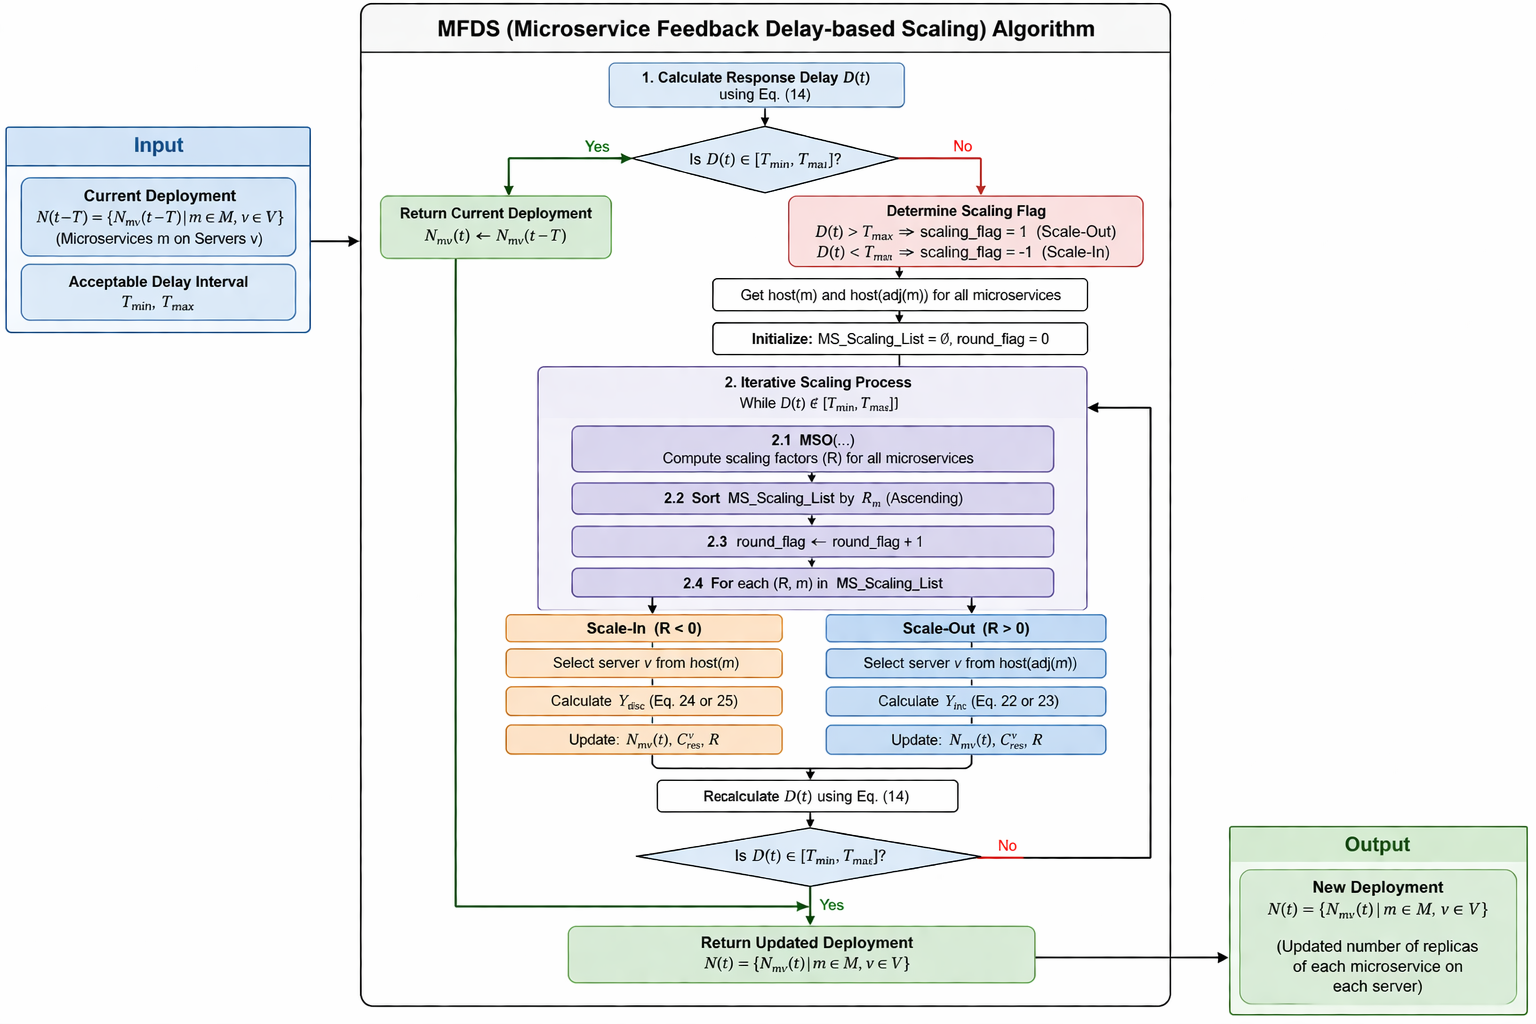
\includegraphics[width=0.9\linewidth]{3/MFDS_ALGOGITHM.png}
\caption{MFDS Algorithm}
\label{fig:sample}
\end{figure}

\pagebreak

\section{MICROSERVICE SCALING OPTIMIZATION (MSO)}

The Microservice Scaling Optimization (MSO) module enhances the efficiency of scaling decisions by computing the optimal number of replicas required for each service in a single calculation step. Unlike traditional incremental scaling approaches that add or remove instances one at a time, MSO directly calculates the target number of instances based on current workload conditions and queuing theory parameters. This optimization uses the relationship between arrival rate ($\lambda$), desired response time, and service capacity to determine the minimum number of servers ($c$) required to meet SLA requirements.

The MSO algorithm evaluates the current system state including request arrival rate, service processing capacity, and target performance metrics to compute the optimal replica count. It considers factors such as expected queue length, system utilization, and response time constraints to ensure that the calculated number of instances can handle the predicted workload while maintaining performance objectives. This mathematical approach eliminates the guesswork involved in incremental scaling and provides precise resource allocation.

This approach significantly minimizes scaling delay and ensures that the system quickly adapts to changing traffic patterns without the iterative overhead of traditional scaling methods. By maintaining optimal utilization levels through precise replica calculation, MSO helps in reducing resource wastage during over-provisioning scenarios while ensuring consistent performance during high-demand periods, ultimately improving both cost efficiency and user experience.

\pagebreak

\begin{figure}[h]
\centering
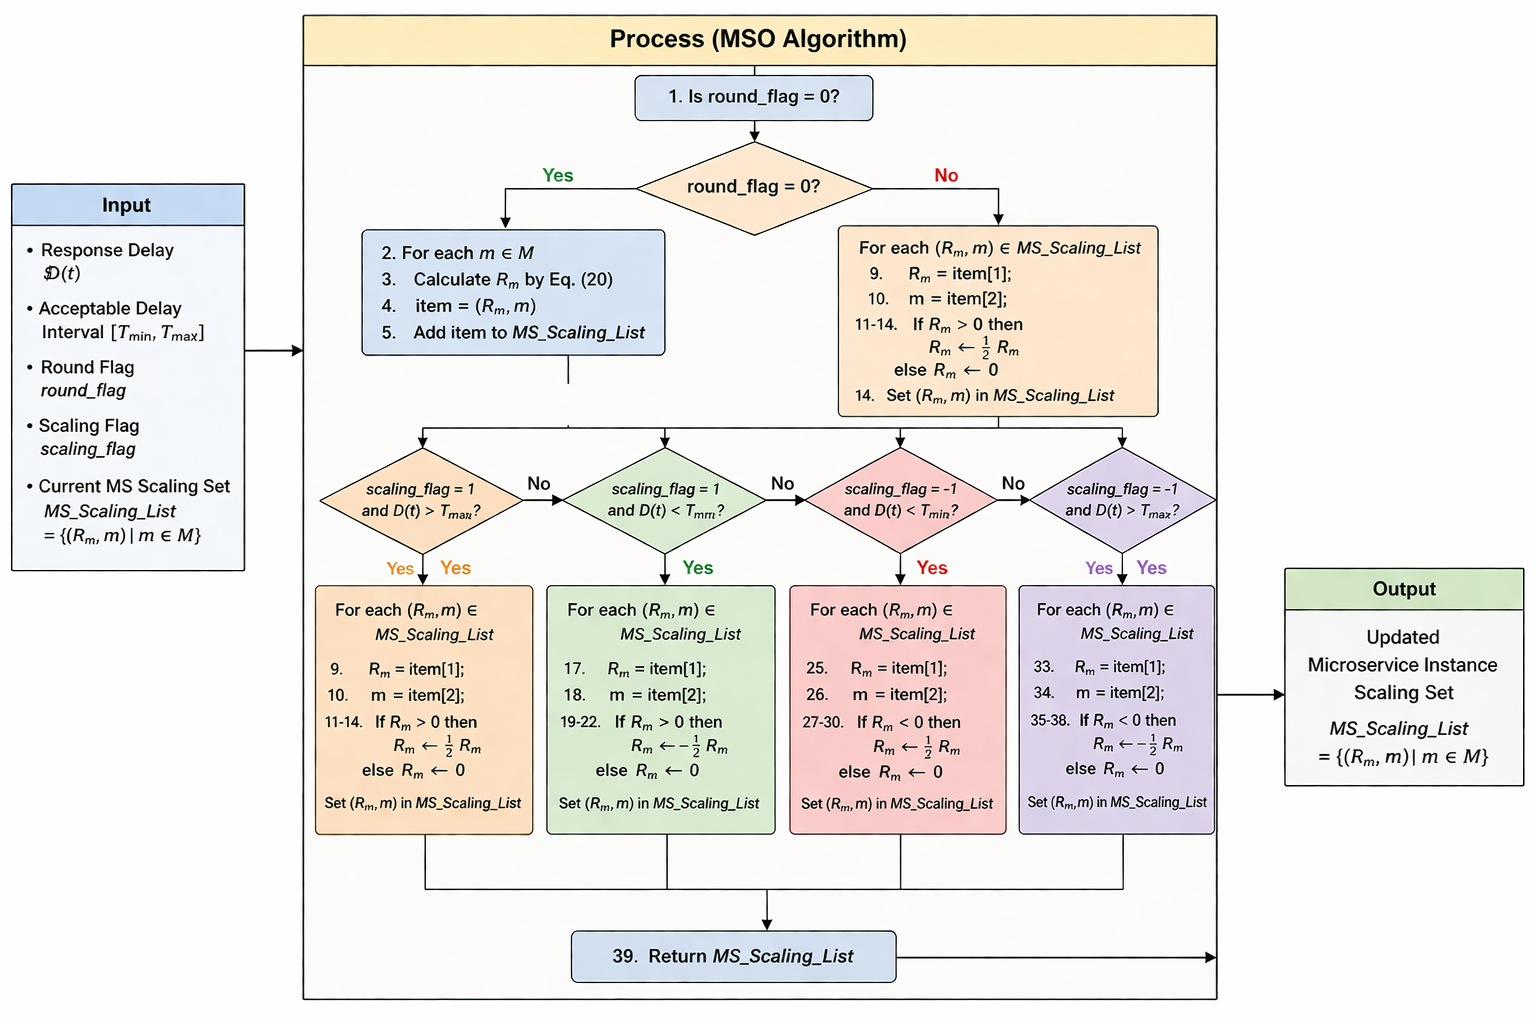
\includegraphics[width=0.7\linewidth]{3/MSO.png}
\caption{MSO Algorithm}
\label{fig:sample}
\end{figure}

\section{FAIR PROBABILISTIC ROUTING (FPR)}

The Fair Probabilistic Routing (FPR) module is responsible for intelligently distributing incoming requests across available service replicas based on real-time system conditions. Unlike traditional round-robin or random routing approaches, FPR calculates dynamic routing probabilities that consider both the number of available replicas and the current workload characteristics of each service instance. The algorithm evaluates factors such as current queue length, processing capacity, and response time to determine optimal traffic distribution patterns.

The routing probabilities are continuously updated based on real-time metrics collected from each service replica, ensuring that traffic allocation adapts to changing system conditions. FPR uses a weighted probability distribution where instances with lower current load and better performance metrics receive higher routing weights, while overloaded instances receive proportionally less traffic. This dynamic adjustment mechanism ensures balanced resource utilization across all available service instances.

This intelligent load distribution ensures that traffic is evenly distributed according to actual service capacity rather than simple numerical equality, preventing overload on individual instances while maximizing overall system throughput.

\begin{figure}[h]
\centering
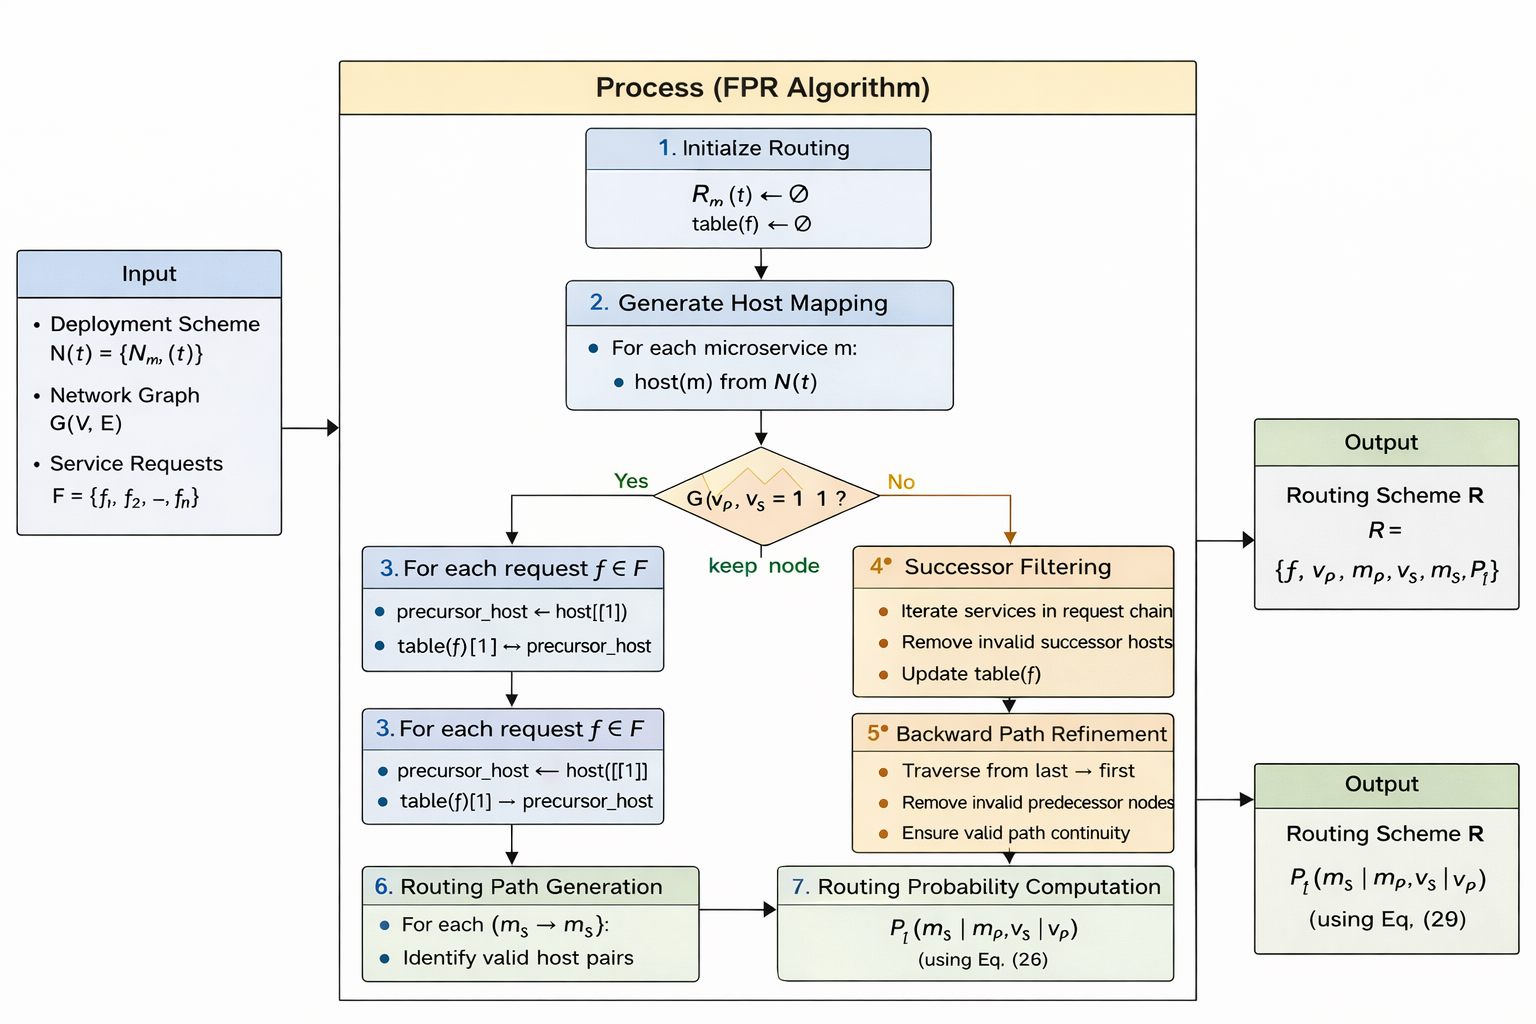
\includegraphics[width=0.7\linewidth]{3/FPR.png}
\caption{FPR Algorithm}
\label{fig:sample}
\end{figure}

\section{DOCKER SWARM SCALING}

Docker Swarm serves as the container orchestration platform responsible for managing and dynamically scaling the microservices infrastructure. Each service in the course registration system (authentication, course catalog, and seat reservation) runs as containerized applications within the Swarm cluster, providing isolation, portability, and consistent deployment environments. The Swarm manager nodes coordinate service deployment and maintain the desired state of each service based on scaling decisions.

The autoscaling engine integrates directly with Docker Swarm's API to execute scaling actions determined by the MFDS and MSO algorithms. When scaling decisions are made, the engine issues Docker service update commands to adjust the number of replicas for specific services, such as docker service scale auth-service=5 to scale the authentication service to five replicas. This integration enables automated and real-time scaling of services without manual intervention, ensuring that resource adjustments happen seamlessly in response to changing workload conditions.

Docker Swarm provides additional benefits including built-in load balancing through its ingress network, automatic service discovery that allows services to communicate regardless of their physical location within the cluster, and health monitoring that automatically replaces failed containers. The platform also ensures high availability through leader election and distributed consensus mechanisms, while optimizing resource utilization by efficiently distributing containers across available nodes in the cluster based on resource constraints and placement policies.

\section{REAL-TIME WORKLOAD SIMULATION}

To evaluate the performance of the autoscaling system, a comprehensive traffic simulation module is implemented to generate realistic workload patterns that mirror real-world course registration scenarios. The simulation incorporates multiple distinct phases including baseline load periods (2 req/s for 2 minutes), moderate ramp-up phases (25 req/s for 2 minutes), peak enrollment periods (50 req/s for 3 minutes), gradual ramp-down phases (25 req/s for 2 minutes), and extended cooldown periods (2 req/s for 3 minutes). This structured approach simulates the typical traffic patterns experienced during university registration cycles.

These carefully designed varying workloads help in comprehensively analyzing system behavior under different stress conditions and validating the effectiveness of the MFDS, MSO, and FPR mechanisms across the entire operational spectrum. The simulation generates controlled traffic that exercises the complete service chain from authentication through course selection to seat reservation, enabling thorough evaluation of scaling coordination across interdependent services. The traffic driver ensures that the system performs efficiently under both low-traffic baseline conditions and high-stress peak scenarios, providing insights into scaling responsiveness, resource optimization, and SLA compliance.

The proposed system architecture provides a comprehensive solution for intelligent autoscaling in microservices environments by seamlessly integrating theoretical queuing models with practical cloud deployment systems. By combining real-time Prometheus-based monitoring, queuing-theory-based performance modeling, and dynamic scaling strategies through Docker Swarm orchestration, the system achieves efficient resource utilization and improved performance compared to traditional threshold-based approaches. The integration of MFDS for accurate decision-making, MSO for optimal replica calculation, and FPR for balanced load distribution ensures coordinated scaling actions that maintain system stability while minimizing resource overhead. Overall, the architecture enhances both system stability and scalability under dynamic workload conditions, demonstrating the practical viability of mathematical modeling in operational autoscaling systems.

